% Options for packages loaded elsewhere
\PassOptionsToPackage{unicode}{hyperref}
\PassOptionsToPackage{hyphens}{url}
\documentclass[
  ignorenonframetext,
  aspectratio=169]{beamer}
\newif\ifbibliography
\usepackage{pgfpages}
\setbeamertemplate{caption}[numbered]
\setbeamertemplate{caption label separator}{: }
\setbeamercolor{caption name}{fg=normal text.fg}
\beamertemplatenavigationsymbolsempty
% remove section numbering
\setbeamertemplate{part page}{
  \centering
  \begin{beamercolorbox}[sep=16pt,center]{part title}
    \usebeamerfont{part title}\insertpart\par
  \end{beamercolorbox}
}
\setbeamertemplate{section page}{
  \centering
  \begin{beamercolorbox}[sep=12pt,center]{section title}
    \usebeamerfont{section title}\insertsection\par
  \end{beamercolorbox}
}
\setbeamertemplate{subsection page}{
  \centering
  \begin{beamercolorbox}[sep=8pt,center]{subsection title}
    \usebeamerfont{subsection title}\insertsubsection\par
  \end{beamercolorbox}
}
% Prevent slide breaks in the middle of a paragraph
\widowpenalties 1 10000
\raggedbottom
\AtBeginPart{
  \frame{\partpage}
}
\AtBeginSection{
  \ifbibliography
  \else
    \frame{\sectionpage}
  \fi
}
\AtBeginSubsection{
  \frame{\subsectionpage}
}
\usepackage{iftex}
\ifPDFTeX
  \usepackage[T1]{fontenc}
  \usepackage[utf8]{inputenc}
  \usepackage{textcomp} % provide euro and other symbols
\else % if luatex or xetex
  \usepackage{unicode-math} % this also loads fontspec
  \defaultfontfeatures{Scale=MatchLowercase}
  \defaultfontfeatures[\rmfamily]{Ligatures=TeX,Scale=1}
\fi
\usepackage{lmodern}
\usetheme[]{CambridgeUS}
\usefonttheme[]{structurebold}
\ifPDFTeX\else
  % xetex/luatex font selection
\fi
% Use upquote if available, for straight quotes in verbatim environments
\IfFileExists{upquote.sty}{\usepackage{upquote}}{}
\IfFileExists{microtype.sty}{% use microtype if available
  \usepackage[]{microtype}
  \UseMicrotypeSet[protrusion]{basicmath} % disable protrusion for tt fonts
}{}
\makeatletter
\@ifundefined{KOMAClassName}{% if non-KOMA class
  \IfFileExists{parskip.sty}{%
    \usepackage{parskip}
  }{% else
    \setlength{\parindent}{0pt}
    \setlength{\parskip}{6pt plus 2pt minus 1pt}}
}{% if KOMA class
  \KOMAoptions{parskip=half}}
\makeatother
\usepackage{color}
\usepackage{fancyvrb}
\newcommand{\VerbBar}{|}
\newcommand{\VERB}{\Verb[commandchars=\\\{\}]}
\DefineVerbatimEnvironment{Highlighting}{Verbatim}{commandchars=\\\{\}}
% Add ',fontsize=\small' for more characters per line
\usepackage{framed}
\definecolor{shadecolor}{RGB}{248,248,248}
\newenvironment{Shaded}{\begin{snugshade}}{\end{snugshade}}
\newcommand{\AlertTok}[1]{\textcolor[rgb]{0.94,0.16,0.16}{#1}}
\newcommand{\AnnotationTok}[1]{\textcolor[rgb]{0.56,0.35,0.01}{\textbf{\textit{#1}}}}
\newcommand{\AttributeTok}[1]{\textcolor[rgb]{0.13,0.29,0.53}{#1}}
\newcommand{\BaseNTok}[1]{\textcolor[rgb]{0.00,0.00,0.81}{#1}}
\newcommand{\BuiltInTok}[1]{#1}
\newcommand{\CharTok}[1]{\textcolor[rgb]{0.31,0.60,0.02}{#1}}
\newcommand{\CommentTok}[1]{\textcolor[rgb]{0.56,0.35,0.01}{\textit{#1}}}
\newcommand{\CommentVarTok}[1]{\textcolor[rgb]{0.56,0.35,0.01}{\textbf{\textit{#1}}}}
\newcommand{\ConstantTok}[1]{\textcolor[rgb]{0.56,0.35,0.01}{#1}}
\newcommand{\ControlFlowTok}[1]{\textcolor[rgb]{0.13,0.29,0.53}{\textbf{#1}}}
\newcommand{\DataTypeTok}[1]{\textcolor[rgb]{0.13,0.29,0.53}{#1}}
\newcommand{\DecValTok}[1]{\textcolor[rgb]{0.00,0.00,0.81}{#1}}
\newcommand{\DocumentationTok}[1]{\textcolor[rgb]{0.56,0.35,0.01}{\textbf{\textit{#1}}}}
\newcommand{\ErrorTok}[1]{\textcolor[rgb]{0.64,0.00,0.00}{\textbf{#1}}}
\newcommand{\ExtensionTok}[1]{#1}
\newcommand{\FloatTok}[1]{\textcolor[rgb]{0.00,0.00,0.81}{#1}}
\newcommand{\FunctionTok}[1]{\textcolor[rgb]{0.13,0.29,0.53}{\textbf{#1}}}
\newcommand{\ImportTok}[1]{#1}
\newcommand{\InformationTok}[1]{\textcolor[rgb]{0.56,0.35,0.01}{\textbf{\textit{#1}}}}
\newcommand{\KeywordTok}[1]{\textcolor[rgb]{0.13,0.29,0.53}{\textbf{#1}}}
\newcommand{\NormalTok}[1]{#1}
\newcommand{\OperatorTok}[1]{\textcolor[rgb]{0.81,0.36,0.00}{\textbf{#1}}}
\newcommand{\OtherTok}[1]{\textcolor[rgb]{0.56,0.35,0.01}{#1}}
\newcommand{\PreprocessorTok}[1]{\textcolor[rgb]{0.56,0.35,0.01}{\textit{#1}}}
\newcommand{\RegionMarkerTok}[1]{#1}
\newcommand{\SpecialCharTok}[1]{\textcolor[rgb]{0.81,0.36,0.00}{\textbf{#1}}}
\newcommand{\SpecialStringTok}[1]{\textcolor[rgb]{0.31,0.60,0.02}{#1}}
\newcommand{\StringTok}[1]{\textcolor[rgb]{0.31,0.60,0.02}{#1}}
\newcommand{\VariableTok}[1]{\textcolor[rgb]{0.00,0.00,0.00}{#1}}
\newcommand{\VerbatimStringTok}[1]{\textcolor[rgb]{0.31,0.60,0.02}{#1}}
\newcommand{\WarningTok}[1]{\textcolor[rgb]{0.56,0.35,0.01}{\textbf{\textit{#1}}}}
\usepackage{longtable,booktabs,array}
\usepackage{calc} % for calculating minipage widths
\usepackage{caption}
% Make caption package work with longtable
\makeatletter
\def\fnum@table{\tablename~\thetable}
\makeatother
\setlength{\emergencystretch}{3em} % prevent overfull lines
\providecommand{\tightlist}{%
  \setlength{\itemsep}{0pt}\setlength{\parskip}{0pt}}
\usepackage{booktabs}
\usepackage{xcolor}
\definecolor{burnt}{RGB}{191,87,0}
\definecolor{bggray}{RGB}{245,245,245}
\setbeamercolor{palette primary}{bg=burnt,fg=white}
\setbeamercolor{palette secondary}{bg=burnt!80,fg=white}
\setbeamercolor{palette tertiary}{bg=burnt!60,fg=white}
\setbeamercolor{palette quaternary}{bg=burnt,fg=white}
\setbeamercolor{title}{fg=white,bg=burnt}
\setbeamercolor{subtitle}{fg=white!90}
\setbeamercolor{frametitle}{fg=white,bg=burnt}
\setbeamercolor{block title}{fg=white,bg=burnt}
\setbeamercolor{block body}{fg=black,bg=bggray}
\setbeamercolor{block title alerted}{fg=white,bg=burnt!80}
\setbeamercolor{block body alerted}{fg=black,bg=burnt!10}
\setbeamercolor{itemize item}{fg=burnt}
\setbeamercolor{itemize subitem}{fg=burnt!70}
\setbeamerfont{frametitle}{size=\large,series=\bfseries}
\setbeamerfont{title}{size=\LARGE,series=\bfseries}
\setbeamerfont{block title}{series=\bfseries}
\setbeamertemplate{itemize item}[circle]
\setbeamertemplate{navigation symbols}{}
\setbeamertemplate{footline}[frame number]
\usepackage{bookmark}
\IfFileExists{xurl.sty}{\usepackage{xurl}}{} % add URL line breaks if available
\urlstyle{same}
\hypersetup{
  pdftitle={Credit Card Customer Behavior},
  pdfauthor={Hannia Ashley Alvarado Galván - Santiago Basaldúa Ramírez},
  hidelinks,
  pdfcreator={LaTeX via pandoc}}

\title{Credit Card Customer Behavior}
\subtitle{Hypothesis Testing + Clustering Extension}
\author{Hannia Ashley Alvarado Galván - Santiago Basaldúa Ramírez}
\date{September 01, 2026}

\begin{document}
\frame{\titlepage}

\begin{frame}{Table of Contents}
\protect\phantomsection\label{table-of-contents}
\begin{columns}[T]
\begin{column}{0.5\textwidth}
\textbf{\color{burnt} Part 1: Hypothesis Testing}
\begin{itemize}
  \item[4.] Project Overview
  \item[5.] Data Wrangling with \texttt{dplyr}
  \item[6.] H1 Overview
  \item[7.] H1: Formal Statement
  \item[8.] H1: Exploratory Plots
  \item[9.] H1: Welch's $t$-Test
  \item[10.] H1: Decision \& Interpretation
  \item[11.] H2: Intuitive Claim
  \item[12.] H2: Scatterplot \& Distribution
  \item[13.] H2: Outlier Detection
  \item[14.] H2: Pearson Correlation
\end{itemize}
\end{column}
\begin{column}{0.5\textwidth}
\textbf{\color{burnt} Part 2: K-Means Clustering}
\begin{itemize}
  \item[15.] Key Correlations Found
  \item[16.] Correlation Matrix
  \item[17.] Clustering Extension
  \item[18.] EDA: Key Findings
  \item[19.] Why K-Means?
  \item[20.] K-Means: 5 Customer Groups
  \item[21.] Conclusions
  \item[22.] References
  \item[23.] Project Access (QR)
\end{itemize}
\end{column}
\end{columns}
\end{frame}

\begin{frame}{Meet the Team}
\protect\phantomsection\label{meet-the-team}
\begin{columns}[T]

\begin{column}{0.48\textwidth}
\begin{center}
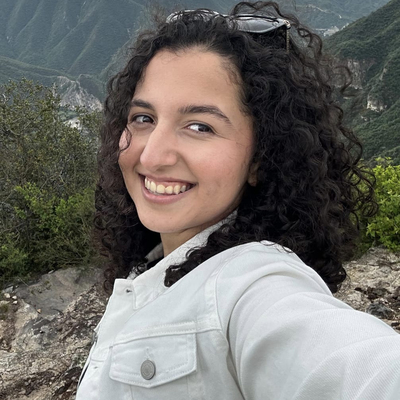
\includegraphics[width=3.0cm, height=3.0cm, keepaspectratio]{a_crop.png}\\[0.4em]
\textbf{Hannia Ashley Alvarado Galv\'{a}n}\\[0.2em]
{\small \texttt{ha26947}}\\[0.4em]
\begin{tabular}{@{}ll@{}}
  {\footnotesize School:} & {\footnotesize UNAM ENES Morelia} \\
  {\footnotesize Major:}  & {\footnotesize Information Technologies} \\
                          & {\footnotesize for Sciences} \\
  {\footnotesize State:}  & {\footnotesize Michoac\'{a}n, M\'{e}xico} \\
\end{tabular}
\end{center}
\end{column}

\begin{column}{0.04\textwidth}\end{column}

\begin{column}{0.48\textwidth}
\begin{center}
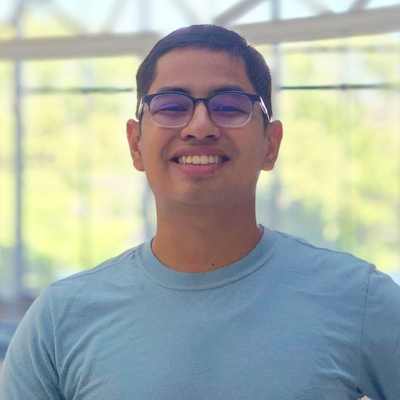
\includegraphics[width=3.0cm, height=3.0cm, keepaspectratio]{b_crop.png}\\[0.4em]
\textbf{Santiago Basald\'{u}a Ram\'{i}rez}\\[0.2em]
{\small \texttt{sb74887}}\\[0.4em]
\begin{tabular}{@{}ll@{}}
  {\footnotesize School:} & {\footnotesize UT Altamira} \\
  {\footnotesize Major:}  & {\footnotesize Mechatronics Engineering} \\
  {\footnotesize State:}  & {\footnotesize Tamaulipas, M\'{e}xico} \\
\end{tabular}
\end{center}
\end{column}

\end{columns}
\end{frame}

\begin{frame}{Project Overview}
\protect\phantomsection\label{project-overview}
\begin{block}{Research Question}
\textit{Do distinct patterns of credit card usage carry statistically measurable
differences, and can we identify natural customer profiles through clustering?}
\end{block}

\vspace{0.4em}

\begin{tabular}{lll}
\toprule
 & \textbf{Part 1} & \textbf{Part 2} \\
\midrule
Approach & Hypothesis Testing & K-Means Clustering \\
Tools & \texttt{t.test()}, \texttt{cor.test()} & \texttt{kmeans()}, \texttt{dplyr} \\
Goal & Confirm or debunk claims & Discover customer groups \\
Dataset & \multicolumn{2}{l}{CC GENERAL --- 8,950 customers, 18 variables} \\
\bottomrule
\end{tabular}

\vspace{0.3em}

\textbf{Significance level for all tests:} \(\alpha = 0.05\)
\end{frame}

\begin{frame}[fragile]{Data Wrangling with \texttt{dplyr}}
\protect\phantomsection\label{data-wrangling-with-dplyr}
\begin{Shaded}
\begin{Highlighting}[]
\NormalTok{cc\_clean }\OtherTok{\textless{}{-}}\NormalTok{ cc }\SpecialCharTok{\%\textgreater{}\%}
  \FunctionTok{filter}\NormalTok{(}\SpecialCharTok{!}\FunctionTok{is.na}\NormalTok{(CREDIT\_LIMIT), }\SpecialCharTok{!}\FunctionTok{is.na}\NormalTok{(MINIMUM\_PAYMENTS)) }\SpecialCharTok{\%\textgreater{}\%}
  \FunctionTok{mutate}\NormalTok{(}
    \AttributeTok{CA\_Group    =} \FunctionTok{if\_else}\NormalTok{(CASH\_ADVANCE\_FREQUENCY }\SpecialCharTok{\textgreater{}=} \FloatTok{0.25}\NormalTok{,}
                          \StringTok{"Heavy CA"}\NormalTok{, }\StringTok{"Light CA"}\NormalTok{),}
    \AttributeTok{LOG\_BALANCE =} \FunctionTok{log1p}\NormalTok{(BALANCE)}
\NormalTok{  )}
\end{Highlighting}
\end{Shaded}

\vspace{0.5em}

\begin{verbatim}
Rows after cleaning: 8636 
\end{verbatim}

\begin{verbatim}

Heavy CA Light CA 
    2204     6432 
\end{verbatim}
\end{frame}

\begin{frame}{Part 1: Hypothesis Testing --- Overview}
\protect\phantomsection\label{part-1-hypothesis-testing-overview}
\begin{block}{H1 -- Heavy Cash-Advance Users Carry Higher Balances}
Test: One-tailed Welch's two-sample $t$-test \hfill \textbf{Expected: Confirmed}
\end{block}

\begin{alertblock}{H2 -- Balance Strongly Predicts Credit Limit (Debunk)}
Test: Pearson correlation \texttt{cor.test()} \hfill \textbf{Expected: Debunked}
\end{alertblock}

\vspace{0.5em}

\begin{longtable}[]{@{}
  >{\raggedright\arraybackslash}p{(\linewidth - 4\tabcolsep) * \real{0.3333}}
  >{\raggedright\arraybackslash}p{(\linewidth - 4\tabcolsep) * \real{0.3333}}
  >{\raggedright\arraybackslash}p{(\linewidth - 4\tabcolsep) * \real{0.3333}}@{}}
\toprule\noalign{}
\begin{minipage}[b]{\linewidth}\raggedright
\end{minipage} & \begin{minipage}[b]{\linewidth}\raggedright
H1
\end{minipage} & \begin{minipage}[b]{\linewidth}\raggedright
H2
\end{minipage} \\
\midrule\noalign{}
\endhead
\textbf{Null Hypothesis} & \(\mu_{\text{Heavy}} = \mu_{\text{Light}}\) &
\(\rho = 0\) \\
\textbf{Alternative} & \(\mu_{\text{Heavy}} > \mu_{\text{Light}}\) &
\(\rho \neq 0\) (strong) \\
\textbf{Key metric} & \(t\)-statistic, \(p\)-value & \(r\), \(r^2\) \\
\bottomrule\noalign{}
\end{longtable}
\end{frame}

\begin{frame}[fragile]{H1: Formal Statement}
\protect\phantomsection\label{h1-formal-statement}
\(\boldsymbol{H_0: \mu_{\text{Heavy CA}} = \mu_{\text{Light CA}}}\)
(\(\mu_{\text{Heavy CA}}\) is the average balance of Heavy CA users, and
it is equal to \(\mu_{\text{Light CA}}\) which is the average balance of
Light CA users)

\vspace{0.5em}

\(\boldsymbol{H_1: \mu_{\text{Heavy CA}} > \mu_{\text{Light CA}}}\)
(\(\mu_{\text{Heavy CA}}\) is the average balance of Heavy CA users, and
it is greater than \(\mu_{\text{Light CA}}\) which is the average
balance of Light CA users)

\begin{block}{Rationale}
The correlation matrix shows
$r(\texttt{BALANCE},\,\texttt{CASH\_ADVANCE\_FREQUENCY}) \approx 0.449$.
Customers who rely on cash advances tend to accumulate higher account balances
(\texttt{BALANCE} = balance amount left in account to make purchases) ---
because cash advances incur high fees and interest immediately upon withdrawal.
\end{block}

\vspace{0.3em}

\textbf{Test chosen:} Welch's two-sample \(t\)-test
(\texttt{var.equal\ =\ FALSE}) --- safe default when group variances
differ.
\end{frame}

\begin{frame}{H1: Exploratory Plots}
\protect\phantomsection\label{h1-exploratory-plots}
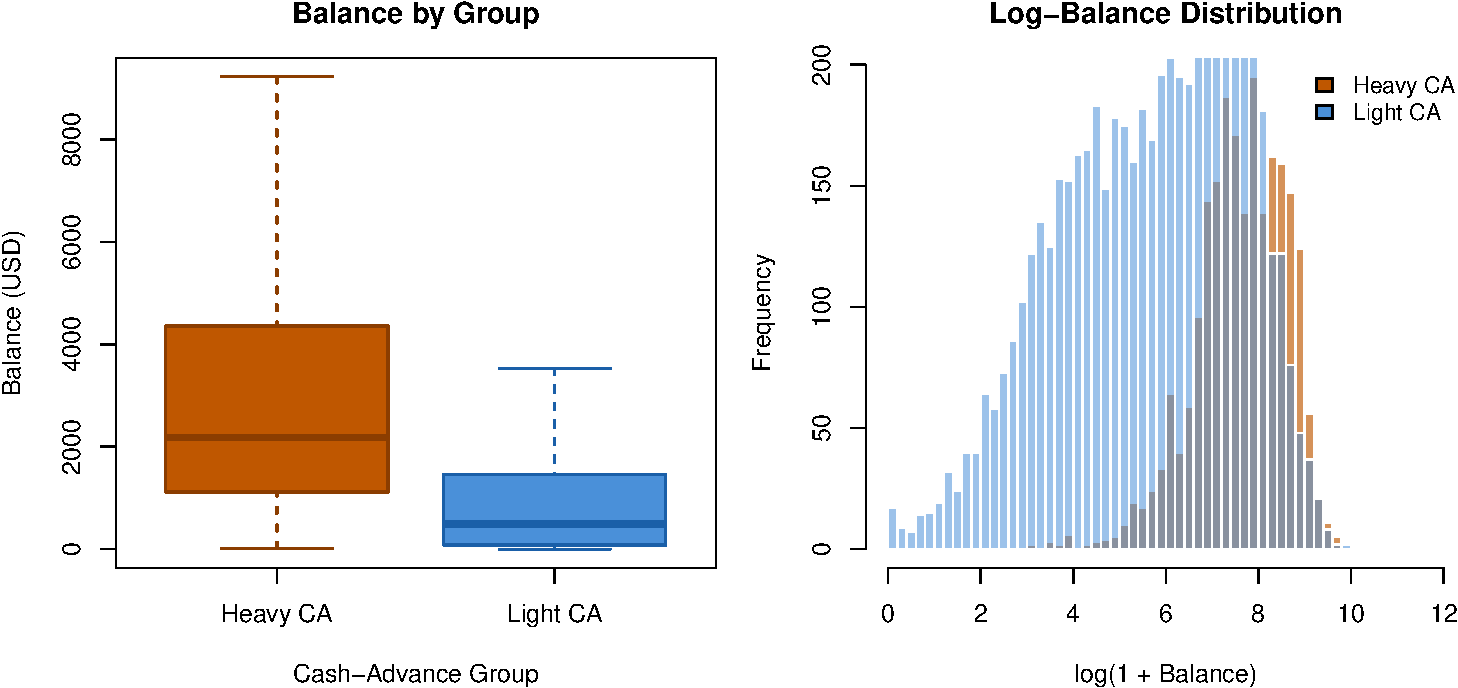
\includegraphics[width=1\linewidth]{presentation_files/figure-beamer/h1-plots-1}
\end{frame}

\begin{frame}[fragile]{H1: Welch's \emph{t}-Test}
\protect\phantomsection\label{h1-welchs-t-test}
\begin{Shaded}
\begin{Highlighting}[]
\NormalTok{t\_result\_h1 }\OtherTok{\textless{}{-}} \FunctionTok{t.test}\NormalTok{(}
  \AttributeTok{x           =}\NormalTok{ heavy,}
  \AttributeTok{y           =}\NormalTok{ light,}
  \AttributeTok{alternative =} \StringTok{"greater"}\NormalTok{,  }\CommentTok{\# one{-}tailed: Heavy \textgreater{} Light}
  \AttributeTok{var.equal   =} \ConstantTok{FALSE}       \CommentTok{\# Welch\textquotesingle{}s t{-}test}
\NormalTok{)}
\end{Highlighting}
\end{Shaded}

\begin{verbatim}
t  = 32.319
\end{verbatim}

\begin{verbatim}
df = 2889.6
\end{verbatim}

\begin{verbatim}
p  = 3.43e-196
\end{verbatim}

\begin{verbatim}
95% CI (lower bound): $1775
\end{verbatim}
\end{frame}

\begin{frame}[fragile]{H1: Decision \& Interpretation}
\protect\phantomsection\label{h1-decision-interpretation}
\begin{verbatim}
t-statistic : 32.319
\end{verbatim}

\begin{verbatim}
p-value     : 3.43e-196
\end{verbatim}

\begin{verbatim}
95% CI lower bound: $1775.11
\end{verbatim}

\begin{verbatim}
Decision    : REJECT H0
\end{verbatim}

\vspace{0.4em}

\begin{block}{Interpretation}
The large positive $t$ and the near-zero $p$-value provide strong statistical
evidence: heavy cash-advance users carry \textbf{significantly higher} balances on average.
CA frequency is a \textbf{measurable financial risk signal}.
\end{block}
\end{frame}

\begin{frame}[fragile]{H2 (Debunk): The Intuitive Claim}
\protect\phantomsection\label{h2-debunk-the-intuitive-claim}
\begin{alertblock}{Common Intuition}
``Customers with higher balances must have higher credit limits ---
the bank gave them more credit, so they use more of it.''
\end{alertblock}

\vspace{0.5em}

\(\boldsymbol{H_0: \rho = 0}\) (\(\rho\) is the correlation between
BALANCE and CREDIT\_LIMIT, and it is equal to zero, meaning there is no
relationship)

\vspace{0.5em}

\(\boldsymbol{H_1: \rho \neq 0}\) (\(\rho\) is the correlation between
BALANCE and CREDIT\_LIMIT, and it is not equal to zero, meaning there is
a strong positive relationship)

\vspace{0.3em}

\textbf{Debunk strategy --- three prongs:}

\begin{enumerate}
\tightlist
\item
  \textbf{Moderate \(r\)} from \texttt{cor.test()} --- \(r^2\) explains
  only \(\approx 29\%\) of variance
\item
  \textbf{Severe outliers} in \texttt{boxplot()} that distort the visual
  pattern
\item
  \textbf{Right-skewed distribution} in \texttt{hist()} --- normality
  assumption violated
\end{enumerate}
\end{frame}

\begin{frame}{H2: Scatterplot \& Distribution}
\protect\phantomsection\label{h2-scatterplot-distribution}
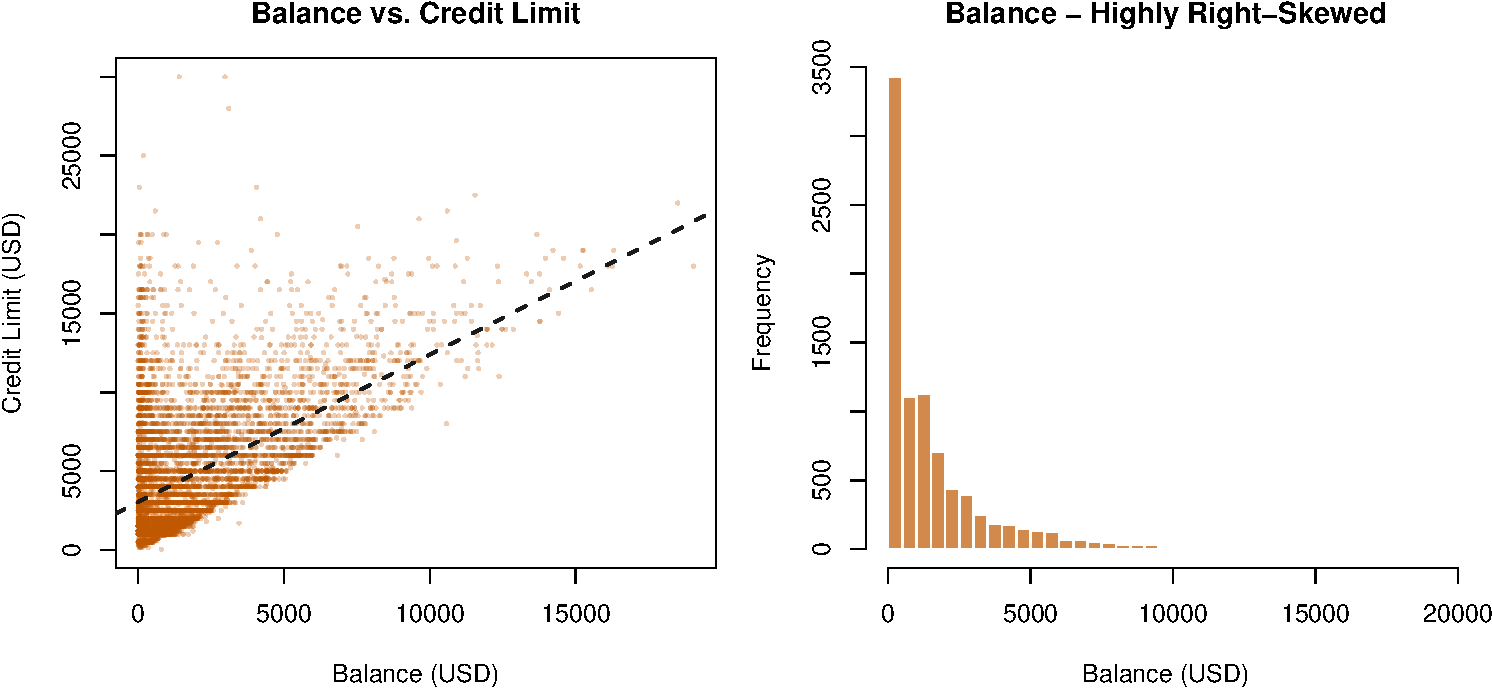
\includegraphics[width=1\linewidth]{presentation_files/figure-beamer/h2-scatter-1}
\end{frame}

\begin{frame}[fragile]{H2: Outlier Detection}
\protect\phantomsection\label{h2-outlier-detection}
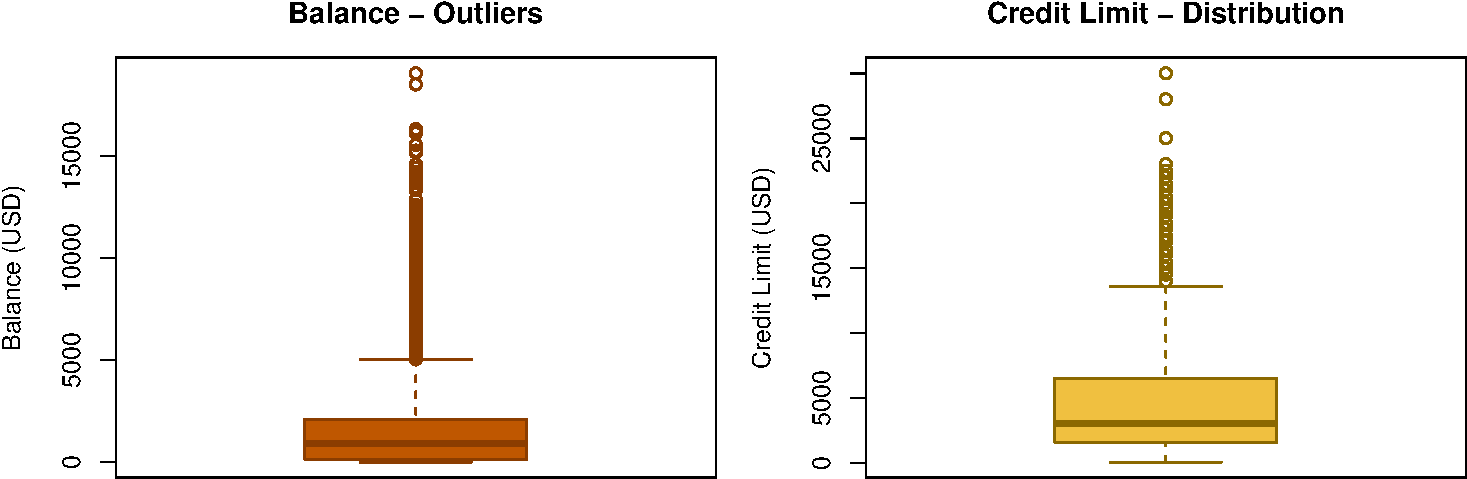
\includegraphics[width=1\linewidth]{presentation_files/figure-beamer/h2-outliers-1}

\begin{verbatim}
Balance outliers (IQR rule): 666 customers
\end{verbatim}
\end{frame}

\begin{frame}[fragile]{H2: Pearson Correlation Test \& Debunk}
\protect\phantomsection\label{h2-pearson-correlation-test-debunk}
\begin{Shaded}
\begin{Highlighting}[]
\NormalTok{cor\_h2 }\OtherTok{\textless{}{-}} \FunctionTok{cor.test}\NormalTok{(cc\_clean}\SpecialCharTok{$}\NormalTok{BALANCE, cc\_clean}\SpecialCharTok{$}\NormalTok{CREDIT\_LIMIT,}
                   \AttributeTok{method =} \StringTok{"pearson"}\NormalTok{)}
\end{Highlighting}
\end{Shaded}

\begin{verbatim}
r (Pearson)         : 0.5355
\end{verbatim}

\begin{verbatim}
r^2 (variance expl.): 28.68%
\end{verbatim}

\begin{verbatim}
p-value             : 0.00e+00
\end{verbatim}

\begin{verbatim}
|r| < 0.35?         : NO  -> DEBUNKED
\end{verbatim}

\begin{alertblock}{Key Lesson: Significance $\neq$ Practical Strength}
With $n = 8{,}950$, even a moderate correlation gives a near-zero $p$-value.
The actual $r \approx 0.54$ seems moderate, but $r^2 \approx 0.29$ means
BALANCE explains only $\approx 29\%$ of CREDIT\_LIMIT variance.
Banks set limits \textit{prospectively} (based on income and credit history),
not in response to current balance --- the strong-prediction claim is \textbf{false}.
\end{alertblock}
\end{frame}

\begin{frame}{Key Correlations Found}
\protect\phantomsection\label{key-correlations-found}
\begin{block}{Three most important relationships}
\begin{itemize}
  \item \textbf{PURCHASES and PAYMENTS} $r \approx 0.60$ (strong positive) ---
        customers who spend more also tend to pay more.
  \item \textbf{CASH\_ADVANCE and BALANCE} $r \approx 0.50$ (moderate positive) ---
        heavier cash-advance use is associated with a higher account balance.
  \item \textbf{PRCFULLPAYMENT and BALANCE} $r \approx -0.32$ (negative) ---
        customers who pay in full carry much lower account balances.
\end{itemize}
\end{block}

\vspace{0.4em}

The matrix also revealed high redundancy between some pairs (e.g.,
PURCHASES and ONEOFF\_PURCHASES: \(r \approx 0.92\)), which guided the
selection of non-overlapping variables for clustering.
\end{frame}

\begin{frame}{Correlation Matrix}
\protect\phantomsection\label{correlation-matrix}
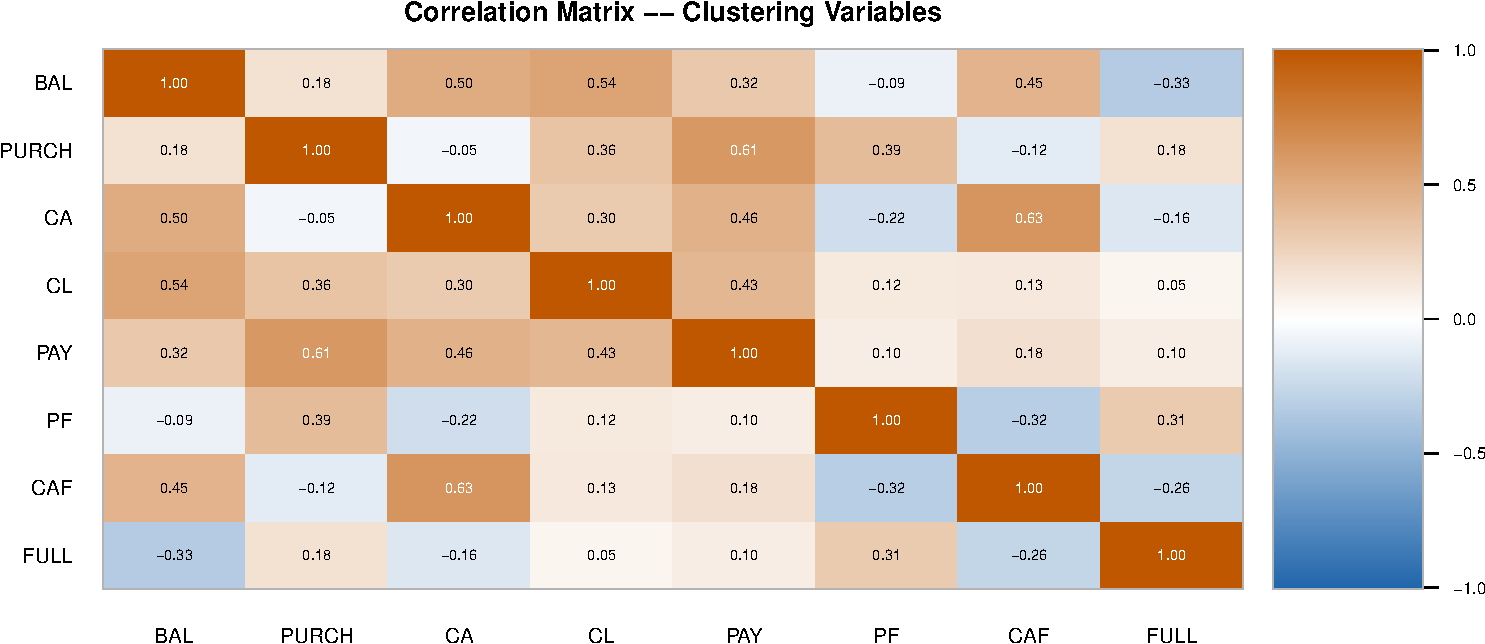
\includegraphics[width=1\linewidth]{presentation_files/figure-beamer/cor-heatmap-1}
\end{frame}

\begin{frame}{Part 2: Clustering Extension}
\protect\phantomsection\label{part-2-clustering-extension}
\begin{center}
\vspace{0.5em}
\large\textbf{Complementary Question:}\\[0.5em]
\normalsize
The hypothesis tests confirmed specific claims about individual variables.\\[0.3em]
Now we ask: \textit{Can we find natural customer groups in the data?}\\[0.6em]
\textbf{Method:} K-Means Clustering --- an exploratory, unsupervised technique\\[0.3em]
\textbf{Input:} 8 financial variables, standardised\\[0.3em]
\textbf{Result:} 5 interpretable customer profiles
\end{center}
\end{frame}

\begin{frame}{EDA: Key Findings}
\protect\phantomsection\label{eda-key-findings}
\begin{columns}[T]

\begin{column}{0.42\textwidth}
\vspace{0.2em}
\begin{itemize}
  \item \textbf{8,950 customers}, 18 variables
  \item All major financial variables are \textbf{strongly right-skewed}:
  \begin{itemize}
    \item PURCHASES: skew = 8.14
    \item CASH\_ADVANCE: skew = 5.17
    \item BALANCE: skew = 2.39
  \end{itemize}
  \item Mean $\gg$ Median for most variables --- a small group of high-activity customers pulls the average up
  \item Extreme values \textbf{kept} --- they represent real, meaningful customer behavior
\end{itemize}
\end{column}

\begin{column}{0.56\textwidth}

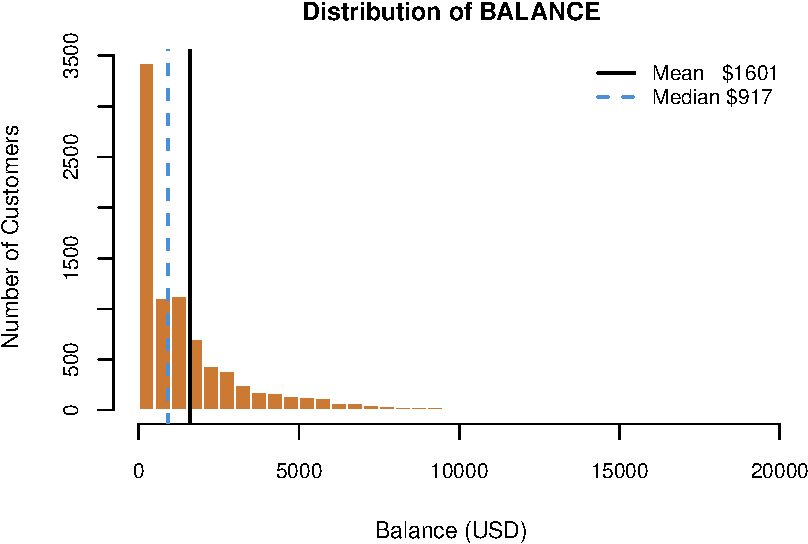
\includegraphics[width=1\linewidth]{presentation_files/figure-beamer/eda-hist-1} 
\end{column}

\end{columns}
\end{frame}

\begin{frame}{Why K-Means Clustering?}
\protect\phantomsection\label{why-k-means-clustering}
\begin{alertblock}{The dataset has no predefined customer categories}
The EDA showed that customers behave very differently from one another.
Clustering groups observations that share similar characteristics,
without requiring a predefined label.
\end{alertblock}

\vspace{0.3em}

\begin{itemize}
  \item \textbf{8 variables} selected: BALANCE, PURCHASES, CASH\_ADVANCE, CREDIT\_LIMIT,
        PAYMENTS, PURCHASES\_FREQUENCY, CASH\_ADVANCE\_FREQUENCY, PRCFULLPAYMENT
  \item Variables were \textbf{standardised} so that dollar-valued variables do not
        dominate frequency variables (0 to 1 scale)
  \item \textbf{K = 5} chosen by comparing several values --- five groups provide
        a useful balance between separation and interpretability
  \item K-Means is used here as an \textbf{exploratory complement} to the
        hypothesis-testing analysis above
\end{itemize}
\end{frame}

\begin{frame}{K-Means Result: 5 Customer Groups}
\protect\phantomsection\label{k-means-result-5-customer-groups}
\begin{tabular}{lcl}
\toprule
Cluster Name & \% Customers & Key Characteristics\\
\midrule
Low-Activity Customers & 38.7\% & Very low purchases, low purchase frequency\\
Regular Purchasers & 32.7\% & Frequent purchases, very low cash-advance use\\
Full-Payment Customers & 14.8\% & Pays full balance consistently, lowest debt carried\\
High Cash-Advance Users & 12.4\% & Very high balance driven by cash advances\\
High-Value Customers & 1.3\% & Extremely high spending and credit limit (n = 112)\\
\bottomrule
\end{tabular}
\end{frame}

\begin{frame}{Conclusions}
\protect\phantomsection\label{conclusions}
\begin{block}{Part 1: Hypothesis Testing}
\begin{itemize}
  \item \textbf{H1 Confirmed} --- Heavy cash-advance users carry significantly higher balances ($p \ll 0.05$). CASH\_ADVANCE\_FREQUENCY is a reliable credit-risk signal.
  \item \textbf{H2 Debunked} --- Despite $p < 0.05$, BALANCE explains only $\approx 29\%$ of CREDIT\_LIMIT variance ($r \approx 0.54$, $r^2 \approx 0.29$). Statistical significance does not imply practical strength.
\end{itemize}
\end{block}

\vspace{0.3em}

\begin{alertblock}{Part 2: Clustering Extension}
K-Means identified \textbf{five interpretable customer profiles} that summarise
different financial behaviors across the 8,950 customers.
These are \textbf{exploratory profiles, not official categories} ---
they complement and contextualise the hypothesis-testing findings above.
\end{alertblock}
\end{frame}

\begin{frame}[fragile]{References}
\protect\phantomsection\label{references}
\vspace{0.5em}

\begin{itemize}
\tightlist
\item
  \textbf{Dataset:} CC GENERAL --- Kaggle Credit Card Customer
  Segmentation (8,950 obs.)
\item
  \textbf{R Packages:} \texttt{dplyr} (wrangling) \(\cdot\) Base R
  (\texttt{stats}, \texttt{graphics})
\item
  \textbf{Statistical Functions:} \texttt{t.test()} \(\cdot\)
  \texttt{cor.test()} \(\cdot\) \texttt{kmeans()}
\item
  \textbf{Visualization:} \texttt{boxplot()} \(\cdot\) \texttt{hist()}
  \(\cdot\) \texttt{plot()} \(\cdot\) \texttt{barplot()} \(\cdot\)
  \texttt{image()}
\item
  \textbf{Concepts Applied:}

  \begin{itemize}
  \tightlist
  \item
    Welch's Two-Sample \(t\)-Test
  \item
    Pearson Correlation --- Effect Size vs.~Significance
  \item
    K-Means Clustering (K = 5, standardised variables)
  \item
    Outlier Detection via IQR Rule
  \end{itemize}
\end{itemize}
\end{frame}

\begin{frame}{Project Access}
\protect\phantomsection\label{project-access}
\begin{center}
\vspace{0.3em}
\large\textbf{Scan for Full Project Materials}\\[0.6em]

\includegraphics[width=4.5cm]{c.png}\\[0.6em]
{\small Full report, presentation source, dataset, and study guide:}\\[0.3em]
\texttt{\small github.com/Sbr0401/FinalBigDataUTEXAS}
\end{center}
\end{frame}

\end{document}
